%!TEX root=../document.tex

\section{Ergebnisse}
\subsection{Theorie}
\subsection{iSCSI Initiator}
\subsection{Client Konfiguration}
\subsection{Server Konfiguration}
\subsection{Testing}
Zuerst wurde mit Client 1 eine Testdatei erstellt. Danach hat Client 2 die Datei geöffnet und bearbeitet.
\begin{figure}[!h]
	\begin{center}
		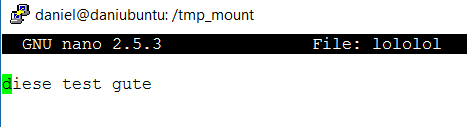
\includegraphics[width=0.5\linewidth]{images/edit.png}
		\caption{Editieren der gemeinsamen Datei}
		\label{edit}
	\end{center}
\end{figure}\

Versucht nun Client 1 ebenfalls die Datei zu editieren erhält man folgende Fehlermeldung:
\begin{figure}[!h]
	\begin{center}
		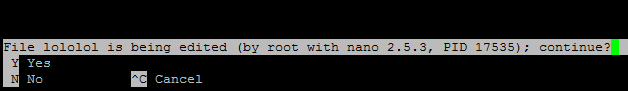
\includegraphics[width=0.8\linewidth]{images/error.png}
		\caption{Gleichzeitiges Editieren}
		\label{error}
	\end{center}
\end{figure}\

Im Endeffekt ist immer die letzte Aktion gültig und überschreibt die vorherigen Änderungen.